\chapter{The Language of Motion}
\label{ch:language}
\begin{chapterintro}
\textbf{You will learn to:} define a reference frame; write the position vector of
a particle; obtain velocity and acceleration by differentiation; eliminate time
to find a trajectory; and interpret motion graphically.
\end{chapterintro}

\section{Reference frame and position}

Motion is always described \emph{relative to a reference frame}. A frame consists
of an origin $O$, a set of axes, and a clock. The position of a material point
$M$ is the vector
\[
\vec{OM}(t)=\vec r(t)=x(t)\ihat+y(t)\jhat+z(t)\khat.
\]
The \textbf{trajectory} is the set of points actually visited. It is obtained by
eliminating the time $t$ from the three parametric equations $x(t),y(t),z(t)$.

A \textbf{material point} is a body whose size is negligible compared with the
distances involved. A train moving between two cities can be a point; a
gymnast rotating about the bar cannot.

\section{Velocity and acceleration}

The average velocity between $t$ and $t+\Delta t$ is
\[
\vec v_{\mathrm{av}}=\frac{\Delta\vec r}{\Delta t}
=\frac{\vec r(t+\Delta t)-\vec r(t)}{\Delta t}.
\]
The instantaneous velocity is the limit:
\[
\vec v(t)=\frac{\dd\vec r}{\dd t}
=\dot x\,\ihat+\dot y\,\jhat+\dot z\,\khat.
\]
The acceleration is the derivative of velocity:
\[
\vec a(t)=\frac{\dd\vec v}{\dd t}
=\frac{\dd^2\vec r}{\dd t^2}
=\ddot x\,\ihat+\ddot y\,\jhat+\ddot z\,\khat.
\]

\begin{keyidea}[Speed versus velocity]
Velocity is a vector. \textbf{Speed} is its magnitude,
$v=\norm{\vec v}=\sqrt{\dot x^2+\dot y^2+\dot z^2}$, and is never negative.
\end{keyidea}

\begin{figure}[htbp]
\centering
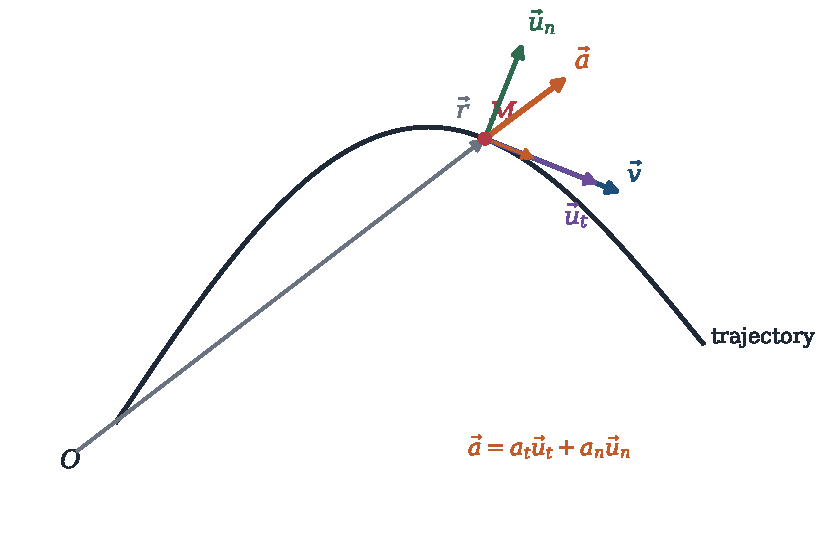
\includegraphics[width=0.88\textwidth]{figures/04_trajectory_frame.pdf}
\caption{At a point of a curved trajectory, the velocity is tangent to the path.
The acceleration generally has a tangential part (changing the speed) and a normal
part (changing the direction).}
\label{fig:trajectory-frame}
\end{figure}

\section{Graphical interpretation}

For one-dimensional motion along $x$:
\begin{itemize}[leftmargin=1.4em,itemsep=3pt]
  \item the slope of the $x$--$t$ graph is the velocity $v=\dd x/\dd t$;
  \item the slope of the $v$--$t$ graph is the acceleration $a=\dd v/\dd t$;
  \item the area under the $v$--$t$ graph is the displacement
        $\Delta x=\int v\,\dd t$;
  \item the area under the $a$--$t$ graph is the change in velocity
        $\Delta v=\int a\,\dd t$.
\end{itemize}

\begin{method}[From acceleration to position]
Given $a(t)$, integrate once to get $v(t)$ and again to get $x(t)$. At each
integration, use the initial conditions $v(0)$ and $x(0)$ to fix the constants.
\end{method}

% ===========================================================================
\section{Worked examples}

\begin{worked}[Position, velocity, acceleration, trajectory]
A particle has position
$\vec r(t)=2t\,\ihat+3t^2\,\jhat+\khat$ (SI units). Find its velocity and
acceleration at $t=1.00\ \mathrm{s}$, its speed, and the equation of its
trajectory.
\end{worked}

\begin{solution}{3.1}
Differentiate component by component:
\[
\vec v(t)=\dot{\vec r}=2\ihat+6t\jhat,\qquad
\vec a(t)=\ddot{\vec r}=6\jhat.
\]
At $t=1$:
\[
\vec v=2\ihat+6\jhat\ \mathrm{m\,s^{-1}},\quad
v=\sqrt{4+36}=6.32\ \mathrm{m\,s^{-1}},
\]
\[
\vec a=6\jhat\ \mathrm{m\,s^{-2}},\quad a=6.00\ \mathrm{m\,s^{-2}}.
\]
For the trajectory, $x=2t$ gives $t=x/2$. Then
\[
y=3t^2=3\left(\frac x2\right)^2=\frac{3x^2}{4},
\]
with $z=1$. The path is a parabola in the horizontal plane $z=1$.
\end{solution}

\begin{worked}[Average versus instantaneous velocity]
A particle moves along the $x$-axis with $x(t)=t^2-4t+3$ (SI units). Find the
average velocity between $t=0$ and $t=3.00\ \mathrm{s}$, and the instantaneous
velocity at $t=1.50\ \mathrm{s}$.
\end{worked}

\begin{solution}{3.2}
\[
x(0)=3,\qquad x(3)=9-12+3=0.
\]
\[
v_{\mathrm{av}}=\frac{x(3)-x(0)}{3-0}=\frac{0-3}{3}=-1.00\ \mathrm{m\,s^{-1}}.
\]
The instantaneous velocity is
\[
v(t)=\dot x=2t-4,
\qquad
v(1.50)=2(1.50)-4=-1.00\ \mathrm{m\,s^{-1}}.
\]
The two happen to be equal here, but they are conceptually different quantities.
\end{solution}

% ===========================================================================
\section{Exercises and Step-by-Step Solutions}

\begin{exercise}{\warm\ Straight-line kinematics}
A particle has position $\vec r(t)=4t\,\ihat+3t^2\,\jhat$ (SI units).
(a) Find $\vec v(t)$ and $\vec a(t)$.
(b) Find the speed at $t=1.00\ \mathrm{s}$.
(c) Find the Cartesian equation of the trajectory.
\end{exercise}

\begin{tabletworkspace}[6.5cm]
\end{tabletworkspace}

\begin{solution}{3.1}
(a)
\[
\vec v=(4,\,6t),\qquad \vec a=(0,\,6).
\]
(b) At $t=1$: $\vec v=(4,6)$, so
$v=\sqrt{16+36}=\sqrt{52}=7.21\ \mathrm{m\,s^{-1}}$.

(c) From $x=4t$, $t=x/4$. Then
\[
y=3\left(\frac x4\right)^2=\frac{3x^2}{16}.
\]
The trajectory is a parabola.
\end{solution}

\begin{exercise}{\warm\ One-dimensional motion}
The position of a particle on the $x$-axis is $x(t)=2t^3-3t^2+1$ (SI units).
(a) Find $v(t)$ and $a(t)$.
(b) Find the velocity and acceleration at $t=2.00\ \mathrm{s}$.
(c) At what times is the particle instantaneously at rest?
\end{exercise}

\begin{tabletworkspace}[6.5cm]
\end{tabletworkspace}

\begin{solution}{3.2}
(a)
\[
v(t)=6t^2-6t=6t(t-1),\qquad a(t)=12t-6.
\]
(b) At $t=2$:
\[
v=24-12=12.0\ \mathrm{m\,s^{-1}},\qquad a=24-6=18.0\ \mathrm{m\,s^{-2}}.
\]
(c) $v=0$ when $6t(t-1)=0$, i.e.\ $t=0$ and $t=1.00\ \mathrm{s}$.
\end{solution}

\begin{exercise}{\warm\ Average velocity}
A particle moves according to $x(t)=5t^2$ (SI units). Compute the average
velocity between $t=1.00\ \mathrm{s}$ and $t=3.00\ \mathrm{s}$, and compare it
with the instantaneous velocity at $t=2.00\ \mathrm{s}$.
\end{exercise}

\begin{tabletworkspace}[6.5cm]
\end{tabletworkspace}

\begin{solution}{3.3}
\[
x(1)=5,\qquad x(3)=45,
\]
\[
v_{\mathrm{av}}=\frac{45-5}{3-1}=20.0\ \mathrm{m\,s^{-1}}.
\]
The instantaneous velocity is $v(t)=10t$, so
$v(2)=20.0\ \mathrm{m\,s^{-1}}$. They are equal because $x\propto t^2$ is
quadratic; the average over a symmetric interval equals the instantaneous value
at the midpoint.
\end{solution}

\begin{exercise}{\core\ Uniform circular motion}
A particle moves in the $xy$-plane with
$\vec r(t)=R\cos(\omega t)\,\ihat+R\sin(\omega t)\,\jhat$, where $R$ and $\omega$
are constants.
(a) Show that the trajectory is a circle.
(b) Find $\vec v(t)$ and show that $\norm{\vec v}=R\omega$.
(c) Find $\vec a(t)$ and show that $\vec a=-\omega^2\vec r$.
\end{exercise}

\begin{tabletworkspace}[6.5cm]
\end{tabletworkspace}

\begin{solution}{3.4}
(a)
\[
x^2+y^2=R^2\cos^2(\omega t)+R^2\sin^2(\omega t)=R^2,
\]
a circle of radius $R$.

(b)
\[
\vec v=-R\omega\sin(\omega t)\,\ihat+R\omega\cos(\omega t)\,\jhat.
\]
\[
\norm{\vec v}=R\omega\sqrt{\sin^2+\cos^2}=R\omega.
\]

(c)
\[
\vec a=-R\omega^2\cos(\omega t)\,\ihat-R\omega^2\sin(\omega t)\,\jhat
=-\omega^2\vec r.
\]
Thus $\norm{\vec a}=R\omega^2$ and the acceleration points toward the centre.
\end{solution}

\begin{exercise}{\core\ Speed and unit tangent}
A particle has position
$\vec r(t)=2t\,\ihat+t^2\,\jhat+\frac{t^3}{3}\,\khat$ (SI units).
Find its velocity, speed, and unit tangent vector at $t=1.00\ \mathrm{s}$.
\end{exercise}

\begin{tabletworkspace}[6.5cm]
\end{tabletworkspace}

\begin{solution}{3.5}
\[
\vec v=(2,\,2t,\,t^2).
\]
At $t=1$:
\[
\vec v=(2,2,1),\qquad v=\sqrt{4+4+1}=3.00\ \mathrm{m\,s^{-1}}.
\]
The unit tangent vector is
\[
\utt=\frac{\vec v}{v}=\left(\frac23,\frac23,\frac13\right).
\]
\end{solution}

\begin{exercise}{\core\ Eliminating time}
A particle moves with $x(t)=2t$ and $y(t)=4t^2-1$ (SI units).
(a) Find the trajectory $y(x)$.
(b) Find $\vec v$ and $\vec a$ at $t=0.50\ \mathrm{s}$.
(c) Is the acceleration constant?
\end{exercise}

\begin{tabletworkspace}[6.5cm]
\end{tabletworkspace}

\begin{solution}{3.6}
(a) From $x=2t$, $t=x/2$, hence
\[
y=4\left(\frac x2\right)^2-1=x^2-1.
\]
This is a parabola opening upward.

(b) $\vec v=(2,8t)$ and $\vec a=(0,8)$. At $t=0.50$:
\[
\vec v=(2,4)\ \mathrm{m\,s^{-1}},\qquad
\norm{\vec v}=\sqrt{20}=4.47\ \mathrm{m\,s^{-1}},
\]
\[
\vec a=(0,8)\ \mathrm{m\,s^{-2}}.
\]
(c) Yes: $\vec a$ is independent of time, so the acceleration is constant.
\end{solution}

\begin{exercise}{\core\ Integrating acceleration}
A particle has acceleration $\vec a(t)=6t\,\ihat$ (SI units), initial velocity
$\vec v(0)=\ihat+2\jhat$, and initial position $\vec r(0)=\vzero$.
Find $\vec v(t)$, $\vec r(t)$, and the position at $t=2.00\ \mathrm{s}$.
\end{exercise}

\begin{tabletworkspace}[6.5cm]
\end{tabletworkspace}

\begin{solution}{3.7}
Integrating $\vec a=6t\,\ihat$:
\[
\vec v(t)=3t^2\ihat+\vec C.
\]
Using $\vec v(0)=\ihat+2\jhat$ gives $\vec C=\ihat+2\jhat$, so
\[
\vec v(t)=(3t^2+1)\ihat+2\jhat.
\]
Integrating again:
\[
\vec r(t)=(t^3+t)\ihat+2t\,\jhat+\vec D.
\]
With $\vec r(0)=\vzero$, $\vec D=\vzero$. Thus
\[
\vec r(t)=(t^3+t)\ihat+2t\,\jhat.
\]
At $t=2$: $\vec r=(8+2)\ihat+4\jhat=10\ihat+4\jhat$ (m).
\end{solution}

\begin{exercise}{\core\ From velocity to position}
A particle has velocity $\vec v(t)=3t^2\,\ihat+2t\,\jhat$ (SI units) and initial
position $\vec r(0)=\ihat$. Find $\vec r(t)$ and the speed at
$t=1.00\ \mathrm{s}$.
\end{exercise}

\begin{tabletworkspace}[6.5cm]
\end{tabletworkspace}

\begin{solution}{3.8}
Integrating $\vec v$:
\[
\vec r(t)=t^3\ihat+t^2\jhat+\vec C.
\]
With $\vec r(0)=\ihat$, $\vec C=\ihat$. Hence
\[
\vec r(t)=(t^3+1)\ihat+t^2\jhat.
\]
At $t=1$:
\[
\vec v=(3,2),\qquad v=\sqrt{9+4}=\sqrt{13}=3.61\ \mathrm{m\,s^{-1}}.
\]
\end{solution}

\begin{exercise}{\mastery\ Helical motion}
A particle moves on the helix
$\vec r(t)=a\cos(\omega t)\,\ihat+a\sin(\omega t)\,\jhat+bt\,\khat$.
(a) Show that its speed is constant.
(b) Find the magnitude of its acceleration.
(c) Describe the direction of the acceleration.
\end{exercise}

\begin{tabletworkspace}[6.5cm]
\end{tabletworkspace}

\begin{solution}{3.9}
(a)
\[
\vec v=-a\omega\sin(\omega t)\ihat+a\omega\cos(\omega t)\jhat+b\khat.
\]
\[
v^2=a^2\omega^2\sin^2+a^2\omega^2\cos^2+b^2
=a^2\omega^2+b^2=\text{const}.
\]
The speed is constant; the velocity direction changes.

(b)
\[
\vec a=-a\omega^2\cos(\omega t)\ihat-a\omega^2\sin(\omega t)\jhat,
\]
so
\[
\norm{\vec a}=a\omega^2.
\]
(c) The acceleration is horizontal and points toward the $z$-axis. It has no
vertical component: the helix is traversed at constant speed and constant
vertical velocity, while the horizontal projection is uniform circular motion.
\end{solution}

\begin{exercise}{\mastery\ Acceleration on a spiral path}
A particle moves in the $xy$-plane with
$\vec r(t)=R\cos(\alpha t^2)\,\ihat+R\sin(\alpha t^2)\,\jhat$, where $R$ and
$\alpha$ are constants.
(a) Find $\vec v(t)$ and $\vec a(t)$.
(b) Identify the tangential and normal components of $\vec a$.
(c) Verify that $a_n=v^2/R$.
\end{exercise}

\begin{tabletworkspace}[6.5cm]
\end{tabletworkspace}

\begin{solution}{3.10}
(a)
\[
\vec v=R(2\alpha t)\bigl[-\sin(\alpha t^2)\ihat+\cos(\alpha t^2)\jhat\bigr].
\]
Differentiating again,
\[
\vec a=R\bigl[-2\alpha\sin(\alpha t^2)-4\alpha^2t^2\cos(\alpha t^2)\bigr]\ihat
+R\bigl[2\alpha\cos(\alpha t^2)-4\alpha^2t^2\sin(\alpha t^2)\bigr]\jhat.
\]

(b) The unit tangent is
$\utt=-\sin(\alpha t^2)\ihat+\cos(\alpha t^2)\jhat$ and the unit normal is
$\un=-\cos(\alpha t^2)\ihat-\sin(\alpha t^2)\jhat$. Therefore
\[
\vec a=\underbrace{2R\alpha}_{a_t}\utt
+\underbrace{4R\alpha^2t^2}_{a_n}\un.
\]
The tangential acceleration is constant, $a_t=2R\alpha$; the normal acceleration
$a_n=4R\alpha^2t^2$ grows with time and points toward the centre (along $\un$).

(c) The speed is $v=2R\alpha t$, so
\[
\frac{v^2}{R}=\frac{4R^2\alpha^2t^2}{R}=4R\alpha^2t^2=\abs{a_n}.
\]
The relation $a_n=v^2/R$ holds, as it must for circular motion of radius $R$.
\end{solution}

